\chapter{Theoretical, computational and experimental methods}


\section{Theoretical principles of molecular dynamics simulations}
%
\begin{quotation}
\textit{[\textcolor{red}{Anfinsen}] showed a film of the folding of a protein with "flickering helices forming and dissolving and coming together to form stable substructures". Of course, the film was purely imaginary, but it led to my asking him whether he had thought of taking the ideas in the film and translating them into a quantitative model. He said that he did not really know how he would do this, but to me it seemed clear that such a model could be based on straightforward physical concepts.} \cite{Karplus:2003aa}
\\
\textit{Martin Karplus}
\end{quotation}
%
%
%
The aim of a molecular dynamics (MD) simulation is to compute the equilibrium and transport properties of a classical many-body system. The term classical means that the interaction between particles and their movement is studied over a given time $t$ through a classical statistical mechanical treatment of the constituent particles. The real power of MD simulations in studying protein dynamics is in the ability to complement experimental studies. MD simulations can act as a figurative \textit{microscope} affording the investigator high spacial and temporal resolution in the study of macromolecular dynamics. Given that most current applications of molecular dynamics simulations of large proteins use a classical statistical mechanical framework due to the enormous computational cost associated with solving the time-dependent Schroedinger equation for biologically interesting molecules, the Hamiltonian of a classical system will be introduced in the following section. This will be followed by a discussion of how molecular forces are computed in an MD simulation, a consideration for how dynamics is calculated in difference physical ensembles and finally, a brief description of the potential energy function used to represent the atomic interaction energies in an MD simulation. 


\subsection{The Hamiltonian of a classical mechanical system}
The Hamiltonian ($H$) can be used to describe a classical system of particles $i$ with coordinates $\mathbf{r}$ and momenta $\mathbf{p}$. The Hamiltonian is equal to the total energy if the potential energy function is independent from time and velocity:
%
%
\begin{equation}
H(\mathbf{r}, \mathbf{p}) \equiv K(\mathbf{p}) + U(\mathbf{r}) = \sum_{i} \frac{\mathbf{p}_{i}^{2}}{2m_{i}} + U(\mathbf{r})
\end{equation}
%
%
where $K$ is the kinetic energy, $U$ is the potential energy and $m$ is the mass. A classical system can therefore be defined by the set of values ${\mathbf{r}, \mathbf{p}}$, which corresponds to a point in phase space defined by the internal coordinates of the system and their momenta. 
%
%
\\\\
%
%
In order to measure thermodynamic averages over a micro-canonical ensemble of states characterised by the macroscopic variables ($N,V,E$), it is necessary to determine the probability distribution of finding the system at each point in phase space ($\rho(\mathbf{r}, \mathbf{p})$). With a knowledge of this distribution of states, one can compute the phase space average of any dynamic variable ($A(\mathbf{r}, \mathbf{p})$) of interest:
%
%
\begin{equation}
\langle A \rangle = \frac{tr \left( e^{- \beta H(\mathbf{r}, \mathbf{p}) } \right) A }{tr \left( e^{- \beta H(\mathbf{r}, \mathbf{p}) } \right) }
\label{equ:classical_ens_obs}
\end{equation}
%
%
where $H$ is the Hamiltonian of the system, $\beta = \frac{1}{k_{B}T}$ and $tr$ is the trace of the operator. With this it is assumed that each quantum state of a many-body system with energy $E$ is equally likely to be occupied. The same thermodynamic observable can be calculated for all quantum states of a system $i$:
%
%
\begin{equation}
\langle A \rangle = \frac{\sum_{i} e^{- \beta E_{i} } < i | A | i > }{\sum_{j} e^{- \beta E_{j} }}
\label{equ:quantum_obs}
\end{equation}
%
%
Unfortunately computing thermal averages for a many-body system by solving the Schroedinger equation and then computing the expectation value of the operator $A$ for all quantum states that have a non-zero statistical weight is not possible for macromolecular systems. The number of quantum states contributing to the operator $A$ in Equ. \ref{equ:quantum_obs} would be so large ($10^{10^{23}}$) that a numerical evaluation of the system would be impractical. For this reason the basic assumption of statistical mechanics is made, whereby it is assumed that a system with fixed number of particles ($N$), volume ($V$) and energy ($E$) is equally likely to be found in any of its quantum states. Such an average over all quantum states of an N-body system in Equ. \ref{equ:classical_ens_obs} is called an \textit{ensemble average}. Nevertheless, in order to compare an observable computed from a simulation with that derived from an experiment, it is desirable to study the time-evolution of that system. Thermal averages can be computed by following the motion of the system through the phase space as a function of time ($t$) by integrating the system's equations of motion, taking the averages only over those points that are visited along the trajectory. Provided that the initial coordinates and momenta of all atoms are defined ($\mathbf{r}^{N}, \mathbf{p}^{N}$), the time-averaged density ($\overline{\rho_{i}(r)}$) can be measured in a molecular dynamics simulation in a volume $V$, at a constant total energy $E$:
%
%
\begin{equation}
\overline{\rho_{i}(r)} = \displaystyle\lim_{t \to \infty} \frac{1}{t} \int_{0}^{t} \: dt' \: \rho_{i}(r;t')
\end{equation}
%
%
The ergodic hypothesis states that when $t$ tends towards infinity and that the trajectory samples the entire phase space, the time average does not depend on the initial conditions. Therefore, averaging over all initial phase space coordinates is equivalent to averaging over the time-evolved space coordinates:
%
%
\begin{equation}
\overline{\rho_{i}(r)} = \langle \rho_{i}(r) \rangle_{NVE}
\label{equ:ergodic_hyp}
\end{equation}
%
%
Generally the above is not true due to the finite length of molecular dynamics simulations, which is constrained by computer processing speed. As such, ergodicity is unattainable for simulations of macromolecules in the vast majority of cases. The ideal simulation length depends primarily on the time-scale of the phenomena of interest. Taking the intrinsic dynamic motion of protein atoms as an example, different atomic and molecular motions are dispersed across a wide range of time scales. The positions of amino acid side chains may fluctuate with a relatively with relatively high frequency (on the ps time scale), whereas large inter-domain tertiary structural rearrangements of the entire protein may occur on much longer time scales (approaching the $\mu$s to ms time scales). In reality, the time scales of these motions largely varies from protein to protein and may depend on the physical and chemical properties of the polypeptide chain. Nevertheless, slow structural dynamics and hence long time scales, still represent a significant computational cost. Apart from using a 'brute-force' approach, this can be overcome by decreasing the number of degrees of freedom of the system, or by biasing the energetic landscape such that the protein is able to traverse free energy barriers and explore conformational space otherwise inaccessible. Neither of these approaches are the subject of this thesis and, as such, will not be reviewed here.


\subsection{The force calculation and integrating the equations of motion}
To start a molecular dynamics simulation, it is first necessary to assign the initial positions and velocities to all particles of the system. Following this initialisation step, the forces on each particle within the system can be calculated and Newton's equations of motion can be solved.  The positions of the atoms are adjusted such that steric clashes between the composite particles are minimised. Additionally, prior to the start of the simulation, velocities are assigned to each particle such that the total momentum is zero and that the instantaneous temperature $T$ matches a desired value:
%
%
\begin{equation}
k_{B}T(t) \equiv \sum^{N}_{i=1} \frac{mv^{2}_{i}(t)}{N_{f}}
\end{equation}
%
%
Next, the forces acting on each of the particles in the system are computed. The forces are subsequently used, along with the positions of the particles at the current and at the previous step, in order to predict the positions at the next step. If a given pair of particles are close enough to interact, the forces along the $x$-direction between these particles are derived from the potential energy ($U(\mathbf{r}^{N})$):
%
%
\begin{equation}
f_{x}(\mathbf{r}) = -\frac{\partial U(\mathbf{r})}{\partial x}
\label{equ:force_calc}
\end{equation}
%
%
The potential energy between each interacting particle in the system is defined by empirically-defined force field potentials. The functional form of these potentials will be described later. It is worth mentioning here that the force evaluation is the most time-consuming step of a molecular dynamics simulation, as it is necessary to consider the contribution to the force on particle $i$ due to all its neighbours. Considering only the interaction between a particle and the nearest image of another particle, it is necessary to evaluate $N \cdot \frac{N-1}{2}$ pair distances, which scales as $N^{2}$. 
%
%
\\\\
%
%
Having computed all the forces for each of the constitutive particles of the system, Newton's equations of motion can be integrated. The simplest way to construct an integrator is through a Taylor expansion of the positions and velocities:
%
%
\begin{equation}
r(t + \Delta t) = r(t) + v(t) \Delta T + \frac{f(t)}{2m} \Delta t^{2} + \frac{\Delta^{3}}{3!} \dddot{r} + O(\Delta t^{4}) 
\end{equation}
%
%
%
%
\begin{equation}
r(t - \Delta t) = r(t) - v(t) \Delta T + \frac{f(t)}{2m} \Delta t^{2} - \frac{\Delta^{3}}{3!} \dddot{r} + O(\Delta t^{4}) 
\end{equation}
%
%
%
%
\begin{equation}
r(t + \Delta t) \simeq 2r(t) - r(t - \Delta t) + \frac{f(t)}{m} \Delta t^{2}
\end{equation}
%
%
These equations have been modified to make them time-reversible \cite{Martyna:1996aa}, thus increasing the accuracy and robustness of the integration. 

\subsection{Molecular dynamics in various ensembles}
Until this point, concepts for simulating a system in the microcanonical (NVE) ensemble have been introduced. Nevertheless, in order to replicate the conditions of a particular experimental set-up, it is often desirable to perform molecular dynamics calculations in different ensembles (ie. NVT or NPT). Physical and mathematical considerations for simulating in these ensembles will be discussed briefly.

\subsubsection{Constant temperature (NVT)}
A constant temperature can be imposed by bringing the system in thermal contact with a large heat bath. This allows for the study of different molecular systems at different temperatures and sampling of the canonical statistical ensemble. Under these conditions, the probability of the system populating a given energy state is given by the Maxwell-Boltzmann velocity distribution:
%
%
\begin{equation}
P(p)=\left( \frac{\beta}{2\pi m} \right) ^{3/2}\cdot exp \left[ \frac{-\beta p^{2}}{2m} \right]
\end{equation}
%
%
We then obtain a simplified relation between the imposed temperature $T$ and the kinetic energy for each particle in the system
%
%
\begin{equation}
k_{B}T=m\langle v^{2}_{\alpha} \rangle
\end{equation}
%
%
where $k_{B}$ is the Boltzmann constant, $m$ is the mass of the particle and $\langle v^{2}_{\alpha} \rangle$ is the time averaged $\alpha$th component of its velocity. This equivalence is often used to measure the temperature of a microcanonical system. Given that the temperature of a system is proportional (though not directly) to the average kinetic energy of the particles, the temperature can be controlled by scaling the velocities. If the temperature at time $t$ is $T(t)$ and the velocities are multiplied by a factor $\lambda$, then the system temperature can be calculated by:
%
%
\begin{equation}
\Delta T=\frac{1}{2} \sum_{i=1} 2\frac{m_{i}(\lambda v_{i})^{2}}{N_{df}k_{B}} - \frac{1}{2} \sum_{i=1} 2\frac{m_{i} v_{i}^{2}}{N_{df}k_{B}}
\end{equation}
%
%
\begin{equation}
\Delta T = (\lambda^{2} -1) T(t)
\end{equation}   
%
%
\begin{equation}
\lambda = \sqrt{\frac{T_{0}}{T(t)}}
\end{equation}
%
%
Multiplying the velocities at each time step by a factor $ \lambda = \sqrt{T_{0}/T(t)} $, where $T(t)$ is the current temperature calculated from the kinetic energy and $T_{0}$ is the desired temperature provides the simplest way of keeping a constant system temperature.
%
%
\\\\
%
%
A simpler formulation of velocity scaling is given by the Berendsen temperature coupling algorithm, in which the velocities are scaled at each step such that the rate of change of the temperature is proportional to the difference in temperature
%
%
\begin{equation}
\frac{dT(t)}{dt} = \frac{1}{\tau}(T_{0}-T(t))
\end{equation}
%
%
where $ \tau $ is a parameter which determines how tightly the system is coupled to the thermal bath. The Berendsen temperature coupling algorithm gives an exponential decay of $ T(t) $ towards $ T_{0} $. The coupling parameter $ \tau $ is given by
%
%
\begin{equation}
\lambda^{2} = 1 + \frac{\delta t}{\tau}\cdot \left[ \frac{T_{0}}{T(t-\frac{\delta t}{2})} -1 \right]
\end{equation}
%
%
In practice the coupling parameter $\tau$ is empirical and the choice of its value alters the strength of coupling between the system and the thermal bath and should be chosen within a reasonable range. Despite the empirical nature of the Berendsen coupling algorithm, it is very efficient for converging systems towards a desired temperature and consequently is commonly used in the equilibration step of an MD simulation \cite{frenkel2001understanding}. Nevertheless, to accurately probe the canonical ensemble, the Extended System approach was first proposed simultaneously by Nos\'{e} \cite{nose1984unified} and Hoover \cite{hoover1985canonical}. The premise of the Nos\'{e}-Hoover approach is to an extended Lagrangian to consider the thermal bath as part of the system by adding a dynamic variable $\tilde{s}$ , which has a non-zero mass and a velocity $\dot{\tilde{s}}$. In the extended system the atomic coordinates are identical to the non-coupled system, however the time scale is stretched by the factor $\tilde{s}$ so that
%
%
\begin{equation}
dt=\tilde{s}dt 
\end{equation}
%
%
The Lagrangian for the extended system is given as
%
%
\begin{equation}
L_{Nose} = \sum_{i=1}^{N}\frac{m_{i}}{2}s^{2}\dot{r}_{i}^{2}-U(r^{2}) + \frac{Q}{2}\dot{s}^{2}  - \frac{L}{\beta} \: ln \: \tilde{s}
\label{equ:nh_lagrangian}
\end{equation}
%
%
where $Q$ is the mass of $\tilde{s}$. The first two terms of the extended Lagrangian represent the potential energy subtracted from the kinetic energy of the real system. The third and forth terms represent the kinetic energy minus the potential energy assigned to $\tilde{s}$. The energy of the real system will fluctuate about a mean and accompanying the fluctuations of $\tilde{s}$, heat transfers occur between the system and the thermal bath, which regulate the system temperature. The momenta conjugate to $\mathbf{r}_{i}$ and $s$ follow directly from Equ. \ref{equ:nh_lagrangian}:
%
%
\begin{equation}
\mathbf{p}_{i} \equiv \frac{\partial L}{\partial \dot{\mathbf{r}}_{i}} = m_{i} s^{2} \dot{\mathbf{r}}_{i}
\end{equation}
%
%
\begin{equation}
p_{s} \equiv \frac{\partial L}{\partial \dot{s}} = Q \dot{s}
\end{equation}
%
%
This gives the extended Hamiltonian of the system if $N$ particles plus the additional coordinate $s$:
%
%
\begin{equation}
H_{Nose} = \sum_{i=1}^{N} \frac{\mathbf{\dot{p}}_{i}^{2} }{2 m_{i} s^{2} } + U \left( \mathbf{r}^{2} \right) + \frac{p_{s}^{2}}{2Q} + L \frac{ln \: s}{\beta}
\end{equation}

\subsubsection{Constant pressure (NPT)}
Many experiments are conducted at a constant pressure, and rather than adjusting the volume of a simulation box in the canonical ensemble, it is often more convenient to ensure a constant pressure. Constant pressure simulations can be attained in the isothermal-isobaric ensemble by considering the volume as a dynamic variable that changes during the simulation. Similar to Hoover scheme to regulate the temperature of the water box, the volume parameter is accounted for by an extended Hamiltonian. The equations of motion for the positions and the momenta are \cite{Martyna:1994aa}:
%
%
\begin{equation}
\mathbf{\dot{r}}_{i} = \frac{\mathbf{p}_{i}}{m_{i}} + \frac{p_{\epsilon}}{W} \mathbf{r}_{i}
\end{equation}
%
%
\begin{equation}
\mathbf{\dot{p}}_{i} = \mathbf{F}_{i} - \left( 1 + \frac{d}{dN} \right) \frac{p_{\epsilon}}{W} \mathbf{p}_{i} - \frac{p_{\xi 1}}{Q_{1}} \mathbf{p}_{i} 
\end{equation}
%
%
where $N$ is the number of particles; the thermostat variable, its momentum and mass are given by $\xi_{1}$, $p_{\xi_1}$ and $Q_{1}$, respectively. This is similar to the thermostat in the Nos\'{e}-Hoover chain algorithm. Additionally, a barostat is introduced via the variables $\epsilon$, $p_{\epsilon}$ and $W$, which give the additional variable, along with its momentum and mass, respectively. The dynamic variable $\epsilon$ that accounts for the barostat is defined as the logarithm of the volume $V$ of the system:
%
%
\begin{equation}
\epsilon = ln \left( \frac{V}{V_{0}} \right)
\end{equation}
%
%
where $V_{0}$ is the volume of the system at time $t=0$. The corresponding equations of motion for the volume are given by:
%
%
\begin{equation}
\dot{V} = \frac{d V p_{\epsilon}}{W}
\end{equation}
%
%
\begin{equation}
\dot{p}_{\epsilon} = dV \left( P_{int} - P_{ext} \right) + \frac{1}{N} \sum_{i=1}^{N} \frac{\mathbf{p}_{i}^{2}}{m_{i}} - \frac{p_{\xi 1}}{Q_{1}} p_{\epsilon}
\end{equation}
%
%
where $P_{ext}$ is the external pressure, which is selected at the outset of the calculation. The internal system pressure of the system ($P_{int}$) is given by:
%
%
\begin{equation}
P_{int} = \frac{1}{dV} \left[ \sum_{i=1}^{N} \left( \frac{\mathbf{p}_{i}^{2}}{m_{i}} + \mathbf{r}_{i} \cdot \mathbf{F}_{i} \right) - dV \frac{\partial U(V)}{\partial V} \right]
\end{equation}
%
%
The Hamiltonian of the extended system is given by:
%
%
\begin{equation}
H_{NPT} = H(\mathbf{p}, \mathbf{r}) + \frac{p_{\epsilon}^{2}}{W} + \sum_{i=1} \frac{p^{2}_{\xi 1}}{Q} + (dN + 1) k_{B}T \: \xi_{1} + k_{B}T \sum_{i=1} \xi_{i} + P_{ext} V
\end{equation}

\subsection{The functional form of the potential energy}
When calculating the forces on each particle $i$ using Equ. \ref{equ:force_calc}, it is necessary to evaluate the potential energy of each interaction in the system. The potential energy between each constitutive particle in a system is represented by an empirically-derived force field potential, which describes the interaction energy between atoms in terms of the atom coordinates ($\mathbf{r}$) and the force field parameters ($s$). The potential energy is written as a sum over different contributions, which can correspond to physical atomic interactions or to unphysical interactions that may be applied to the system:
%
%
\begin{equation}
U(\mathbf{r}; s) = U^{phys}(\mathbf{r}; s) + U^{special}(\mathbf{r}; s)
\end{equation}
%
%
Special unphysical interactions can correspond to restrains to bond lengths and distances, or additional forces applied to the system, though these will not be described here in any further detail. The physical interactions within the system can be further sub-divided into bonded and non-bonded interactions between the composite atoms:
%
%
\begin{equation}
U^{phys}(\mathbf{r}; s) = U^{bonded}(\mathbf{r}; s) + U^{non-bonded}(\mathbf{r}; s)
\end{equation}
%
%
The functional form of the bonded interactions of the Gromos force field parameter set, used herein, are the sum of the bond, bond angle, harmonic dihedral angle and trigonometric dihedral angle terms \cite{Oostenbrink:2004aa}:
%
%
\begin{equation}
U^{bonded}(\mathbf{r}; s) = U^{bond}(\mathbf{r}; s) + U^{bond angle}(\mathbf{r}; s) + U^{harmonic}(\mathbf{r}; s) + U^{trig.}(\mathbf{r}; s)
\end{equation}
%
%
The non-bonded interactions are a sum over the potential associated with van der Waals and electrostatic interactions between all pairs of atoms \cite{Oostenbrink:2004aa}:
%
%
\begin{equation}
U^{non-bonded}(\mathbf{r}; s) = U^{vdW}(\mathbf{r}; s) + U^{electrostatic}(\mathbf{r}; s)
\end{equation}

\subsubsection{Bonded interaction potential}
The energetic potential of covalent bonded interactions is calculated as the sum over all $N_{b}$ bonds and depends on the parameters $K_{b}$ and $b_{0}$, which were originally parametrised against experimental spectroscopic and X-ray diffraction data for small molecules. The functional form of the bonded potential is:
%
%
\begin{equation}
U^{bond}(\mathbf{r}; K_{b}, b_{0}) = \sum_{n=1}^{N_{b}} \frac{1}{2} K_{b_{n}} \left[ b_{n} - b_{0_{n}} \right] ^{2}
\end{equation}
%
%
where $b_{n}$ is the actual bond length, $b_{0}$ is the optimal bond length and $K_{b}$ is the bond force constant. The parameters $K_{b}$ and $b_{0}$ vary depending on the nature of the bonded interaction between given pairs of atoms (\textbf{Fig. \ref{fig:aa_nms} A}). The potential due to the angle between bonded interactions is calculated as a sum of all $N_{\theta}$ bond angles and depends on the parameters $K_{\theta}$ and $\theta_{0}$:
%
%
\begin{equation}
U^{bond angle}(\mathbf{r}; K_{\theta},\theta_{0}) = \sum_{n=1}^{N_{\theta}} \frac{1}{2} K_{b_{\theta}} \left[ cos \: \theta_{n} - cos \: \theta_{0_{n}} \right] ^{2}
\end{equation}
%
%
where $\theta_{n}$ is the actual bond angle, $\theta_{0}$ is the optimal bond angle and $K_{\theta}$ is the bond angle force constant (\textbf{Fig. \ref{fig:aa_nms} B}). The harmonic torsion angles are used to maintain a specific planar configuration for four specific atoms (eg. maintaining a tetrahedral configuration about an sp3 hybridised carbon atom). This potential is calculated as the sum over all improper dihedral interaction centres $N_{\xi}$, with parameters $K_{\xi}$ and $\xi_{0}$ \cite{Oostenbrink:2004aa}:
%
%
\begin{equation}
U^{harmonic}(\mathbf{r}; K_{\xi}, \xi_{0}) = \sum_{n=1}^{N_{\xi}} \frac{1}{2} K_{b_{\xi}} \left[ \xi_{n} - \xi_{0_{n}} \right] ^{2}
\end{equation}
%
%
where $\xi_{n}$ is the actual harmonic torsion (\textbf{Fig. \ref{fig:aa_nms} C}). Similarly, the trigonometric torsion angles are defined as a sum over all $N_{\varphi}$ torsion angles, with parameters $K_{\varphi}$, $\delta$ and $m$:
%
%
\begin{equation}
U^{trig.}(\mathbf{r}; K_{\varphi}, \delta, m) = \sum_{n=1}^{N_{\varphi}} K_{\varphi_{n}} \left[ 1 + cos(\delta_{n}) \: cos(m_{n}\varphi_{n}) \right]
\end{equation}
%
%
where $\delta$ is the phase shift, $m_n$ is the multiplicity of the torsion angle and $\varphi$ is the actual trigonometric torsion angle (\textbf{Fig. \ref{fig:aa_nms} D}). 
%
%
%
%
%%% FIGURE
%
\begin{figure}[!ht]
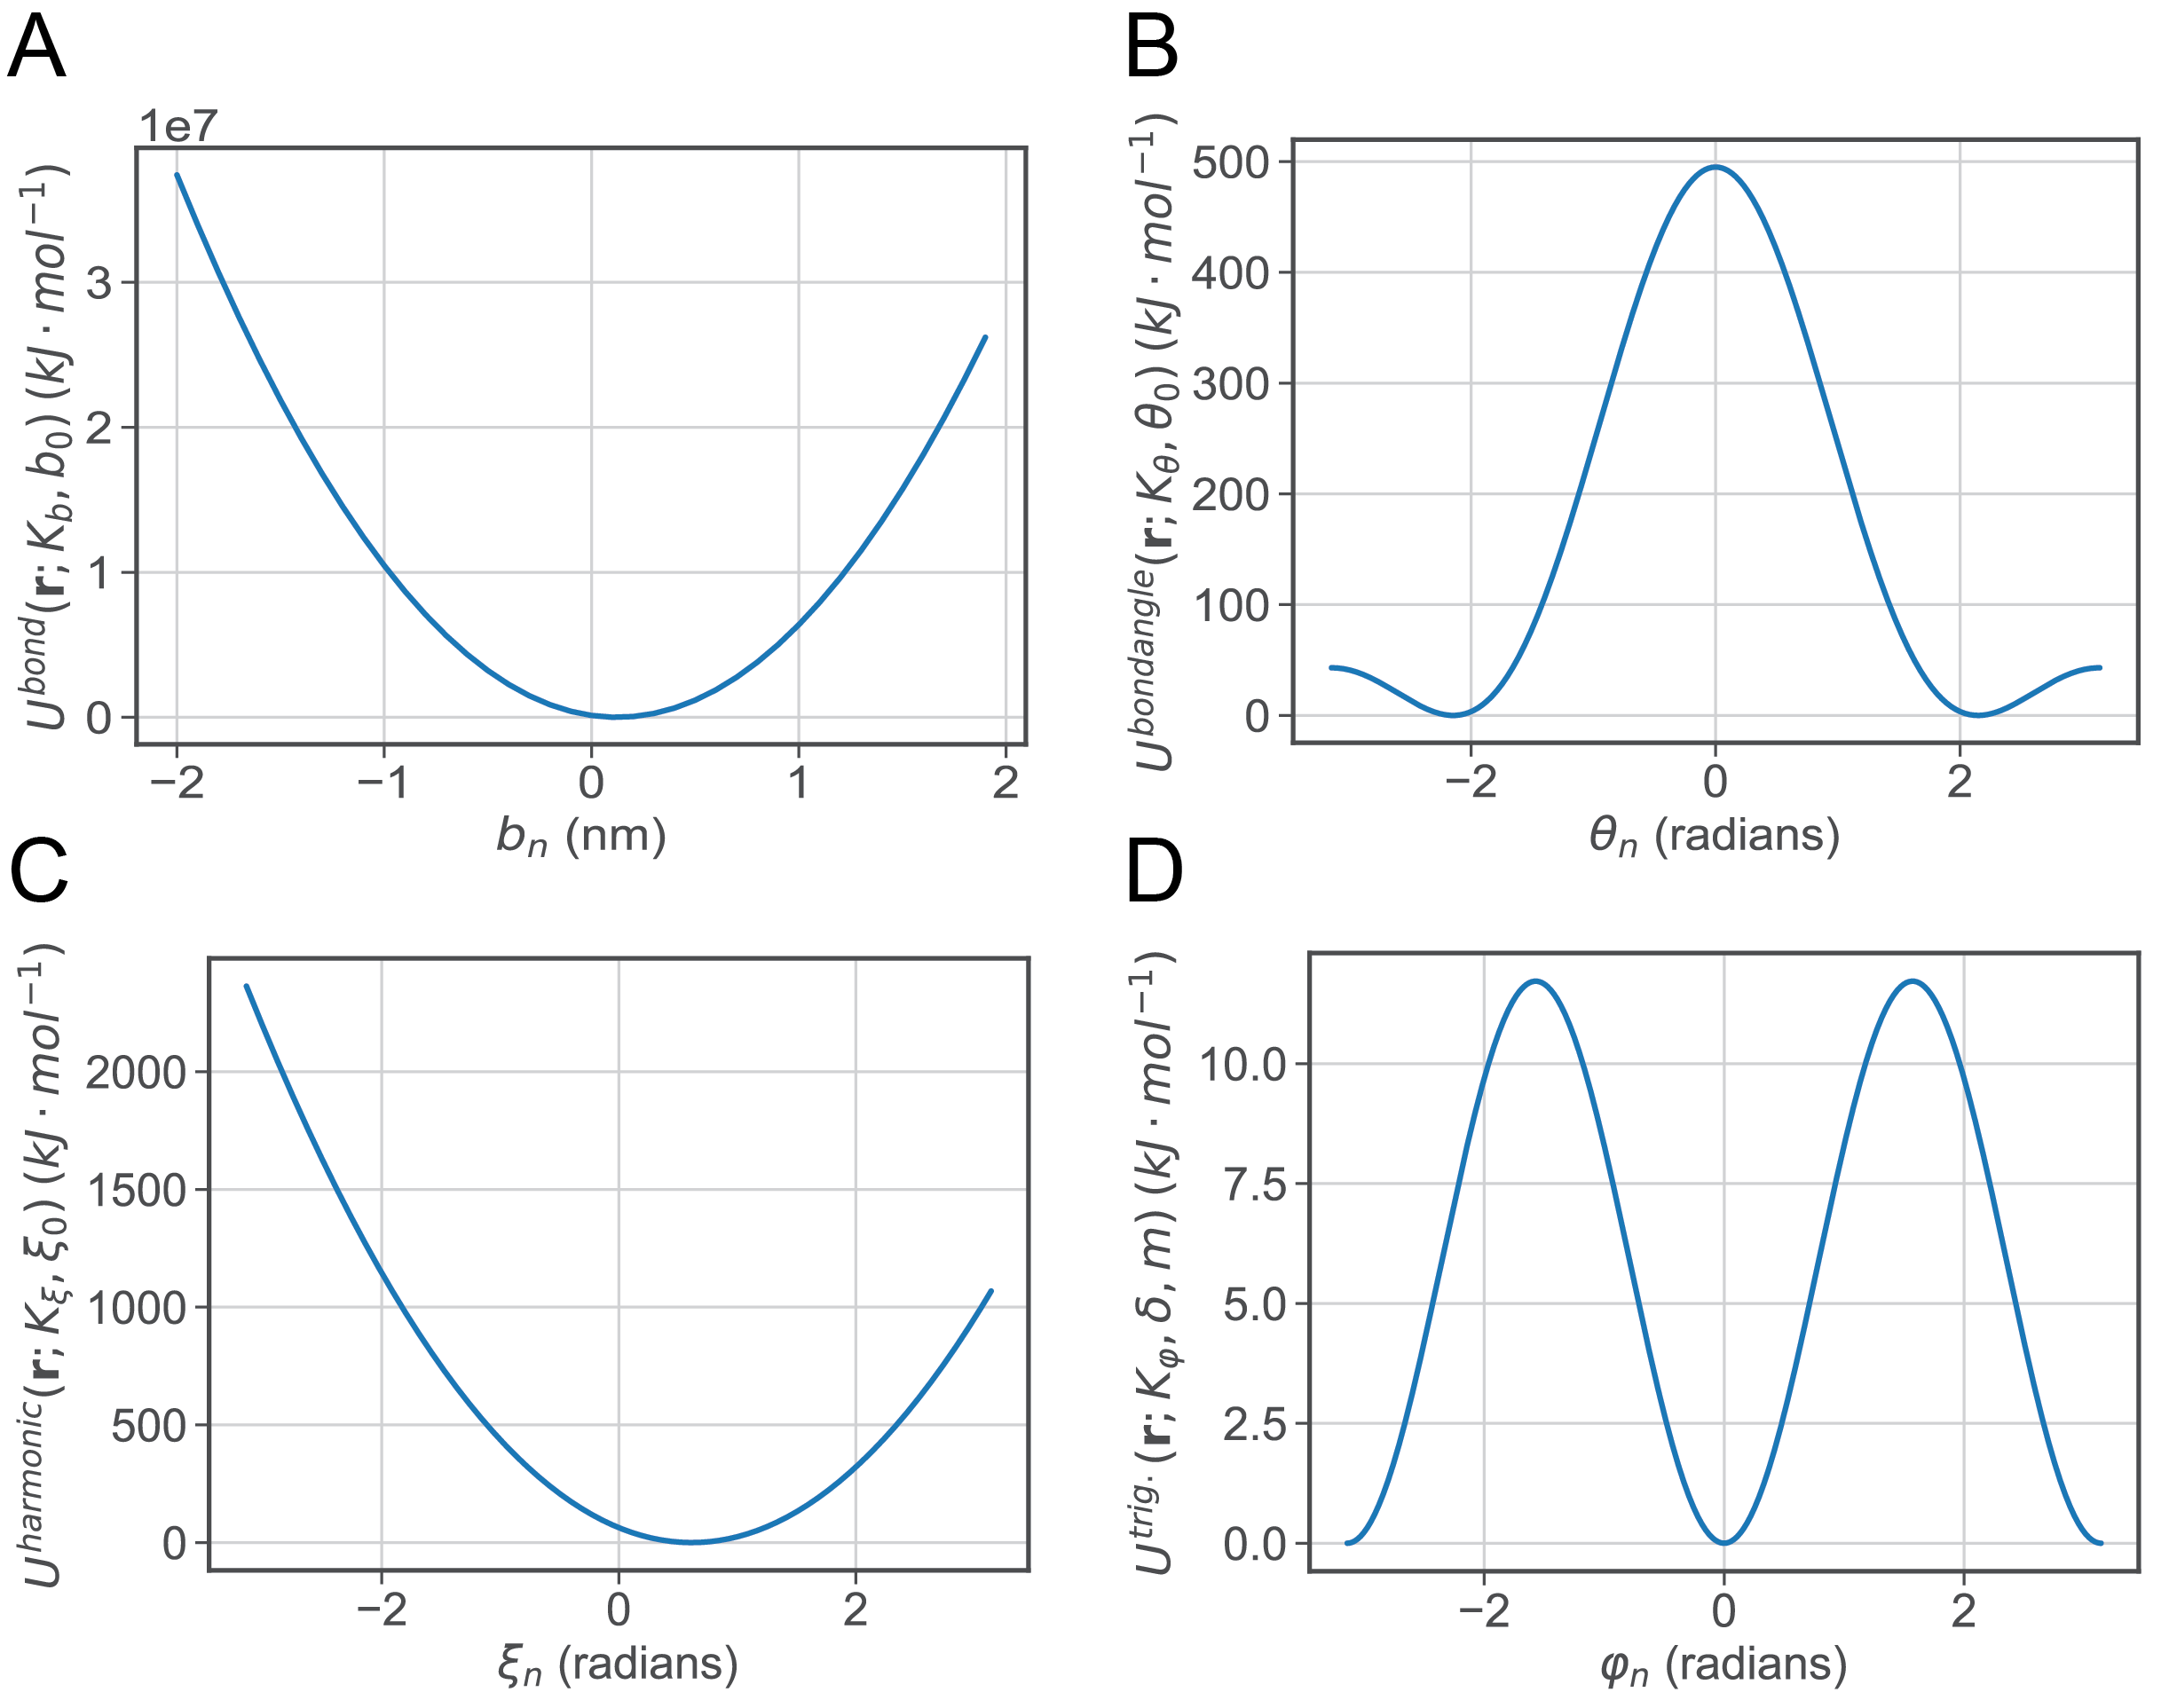
\includegraphics[scale=0.65]{bonded_potential_energy.png}
\caption[Examples of bonded interaction potential energies for arbitrarily selected atom pairs.] {\textbf{Examples of bonded interaction potential energies for arbitrarily selected atoms.} (A) The interaction potential for a C-O bond length. (B) The interaction potential for a H-N-C bond angle. (C) The harmonic torsional potential energy for a tetrahedral centre. (D) The trigonometric torsional potential energy for a -C-C- torsion.}
\label{fig:aa_nms}
\end{figure}
%
%
\clearpage

\subsubsection{Non-bonded interactions}
In the GROMOS force field parameter set, the non-bonded interactions are calculated as the potential between all atoms that are not involved in a covalent (ie. bonded) interaction. There are a number of exceptions to this collection of interactions, including those that fall outside of a defined inter-atomic cut-off range. Two principle non-bonded interaction types are considered: van der Waals interactions and electrostatic interactions. The non-bonded van der Waals potentials are calculated as a sum over all interacting non-bonded atom pairs $i,j$ using a Lennard-Jones 12/6 interaction function with parameters $C12$ and $C6$:
%
%
\begin{equation}
U^{vdW}(\mathbf{r}; C12, C6) = \sum_{i,j} \left( \frac{C12_{i,j}}{r^{12}_{i,j}} - \frac{C6_{i,j}}{r^{6}_{i,j}} \right)
\end{equation}
%
%
Electrostatic interaction potentials are defined as three separate terms: a Coulomb interaction potential, a distance-dependent reaction-field contribution and a distance-independent reaction-field term. The Coulomb potential is given as a sum over all interacting pairs $U^{C}$, with parameters $q$ defined as the partial charges $q_{i}$ on the atoms \cite{Oostenbrink:2004aa}:
%
%
\begin{equation}
U^{C}(\mathbf{r}; q) = \sum_{i,j} \frac{q_{i} q_{j}}{4 \pi \epsilon_{0} \epsilon_{1}} \cdot \frac{1}{r_{ij}}
\end{equation}
%
%
where the dielectric permittivity of a vacuum and that of the solvent in which the atoms are embedded is given by $\epsilon_{0}$ and $\epsilon_{1}$, respectively. In addition to the direct Coulomb interactions, a reaction-field $U^{RF}$ is determined, which represents the interaction of atom $i$ with an induced dielectric field outside a defined cut-off distance $R_{RF}$ in the presence of atom $j$. Finally, a distance-independent reaction-field term is given as a constant contribution to the potential for every pair of atoms taken into account.

\clearpage

\subsubsection{Evaluating long-range electrostatic interactions}
\textcolor{red}{Increasing computational power has allowed for the simulation of ever larger molecular systems. Nevertheless, it is crucial that the computation of all pair interactions is avoided, as otherwise the time complexity of a molecular dynamics algorithm would be proportional to the square of the number of particles. The expense of a molecular dynamics simulation could be reduced rather drastically by truncating the potential of long-range electrostatics, thus assuming that the long-range part of the potential is unimportant. Truncation of long-range electrostatics removes the expensive part of the calculation but introduces serious inaccuracies. Other techniques are available for handling long-range electrostatic interactions and, while more expensive than a simple truncation, have the advantage that they more faithfully respect the long-range character of the forces between a charge-charge pair of atoms. Of the techniques available to evaluate long-range electrostatics, the so-called particle-mesh Ewald summation is often used for biomolecular systems and scales with a time complexity of $\mathcal{O}(n\log{}n)$.
\\
\\
The particle-mesh Ewald scheme is used as a numeric approximation to Ewald summation. In the Ewald summation method, long-range electrostatic interactions are split into two parts: a short-range contribution and a long-range contribution. The short-range contribution is solved in real-space, whereas the long-range contribution is calculated using a Fourier transform. The time complexity for a fully optimised Ewald summation scheme scales to the number of particles as $\mathcal{O}(n^{2/3})$, due to the expense of the reciprocal-space part of the Ewald sum. For the simulation of systems where the number of particles is of the order of $10^5$ it is necessary to have a scheme that handles the Fourier part of the Ewald summation more efficiently. To this end, particle mesh Ewald methods allow for the efficient evaluation of the Fourier part of the Ewald summation scheme by using a so-called Fast Fourier Transform \cite{Darden:1993aa}. First, charged particles are assigned to discrete points on a lattice. Next, a Fast Fourier Transform method is used to compute the Poisson equation for the discrete charge distribution on the defined lattice. Once Poisson equation has been computed to give the electrostatic energy, the forces are calculated and assigned back to the particles on the system.}


\section{Parameters used for molecular dynamics simulations of PKM2}
Molecular dynamics (MD) simulations were used throughout this study to characterise the functional dynamics of PKM2 in explicit solvent and \textit{in vacuo}. 

\subsection{Molecular dynamics simulations in explicit solvent}
MD simulations of monomeric and tetrameric human PKM2 were performed with the GROMACS 5.2 engine \cite{Van-Der-Spoel:2005aa}, in SPC-E water \cite{berendsen1987missing}. Interactions between protein atoms and solvent were modelled using the Gromos 53a6 force field parameter set \cite{Oostenbrink:2004aa}. The input coordinates for monomeric PKM2 in the \textit{apo} form (mPKM2$^{apo}$) were extracted from the Protein Data Bank crystal structure structure 3bjt \cite{Christofk:2008aa}. Coordinates for mPKM2$^{Phe}$ were extracted from 4fxj \cite{Morgan:2013aa};  mPKM2$^{FBP}$, tPKM2$^{FBP}$ and mPKM2$^{Tepp-46}$ from 3u2z \cite{Anastasiou:2012aa}; and coordinates for tPKM2$^{FBP+Phe}$ and tPKM2$^{FBP+Ser}$ were extracted from 4b2d \cite{Chaneton:2012aa}. Missing residues were modelled using holomogy modelling within the Modeller suite \cite{fiser2003modeller}. The force-field parameters for FBP and Tepp-46 were determined using a quantum mechanical assignment of the partial charges using the ATB server \cite{Malde:2011aa}. Structures were solvated in a dodecahedral period box, such that the distance between any protein atom and the periodic boundary was a minimum of 1.0 nm. The system charge was neutralised by adding counter ions to the solvent (Na$^{+}$ and Cl$^{-}$). Equations of motion were integrated using the leap-frog algorithm with a 2 fs time step. The system was equilibrated for 5 ns in the NVT ensemble at 300 K and 1 bar. This was followed by a further 5 ns equilibration in the NPT ensemble. Following equilibration, multiple replicate production run simulations were performed for 400 ns under constant pressure and temperature conditions, 1 bar and 300 K. Temperature was regulated using the velocity-rescaling algorithm, with a coupling constant of 0.1. Covalent bonds and water molecules were restrained with the LINCS \cite{Hess:2008ab} and SETTLE \cite{Miyamoto:1992aa} methods, respectively. Electrostatics were calculated with the particle mesh Ewald method \cite{Darden:1993aa}, with a 1.4 nm cut-off, a 0.12 nm FFT grid spacing and a four-order interpolation polynomial for the reciprocal space sums.

\subsection{Molecular dynamics simulations \textit{in vacuo}}
\label{methods:vacuo_md}
Structural models of the 15+ monomer, 23+ A-A' and C-C' dimers and 33+ tetramers were generated from the PDB crystal structure 3bjt \cite{Christofk:2008aa} by randomly assigning positive charges to histidine residues distributed throughout the protein. Models were simulated in vacuo using the OPLS- AA/L force-field parameter set \cite{Robertson:2015aa}. Systems were minimised using the Steepest Descent algorithm for 5 x 106 steps, with a step size of 1 J mol$^{-1}$ nm$^{-1}$ and a maximal force tolerance of 100 kJ mol$^{-1}$ nm$^{-1}$. Next, systems were equilibrated at consecutively increasing temperatures (100 K, 200 K and 300 K) each for 5 ns, with the Berendsen temperature coupling method and an integration step size of 1 fs. Production run simulations were performed for 10 ns with an integration step size of 2 fs in the canonical ensemble. Pressure coupling and electrostatics were turned off. Temperature was held constant at 300 K using the Berendsen coupling method. The most prevalent structures were extracted using the GROMOS clustering algorithm \cite{Daura:2001aa}. Theoretical collision cross sections were calculated for each clustered structure, using the projection approximation method, as outlined by Ruotolo (2008) \textit{et al.} \cite{Ruotolo:2008aa}, and using the exact hard-sphere scattering model, as implemented in the EHSSrot software \cite{Shvartsburg:2007aa}.

\clearpage

\section{Protein biophysics}

\subsection{Recombinant protein expression and purification}
PKM2 single-point mutant plasmids were generated through a single-step PCR reaction using hot-start KOD polymerase (Merck Millipore; Burlington MA, USA) and a pET28a-His-PKM2(WT) template plasmid (plasmid no. 42515 AddGene; Cambridge MA, USA). Plasmids were sequence-verified by Sanger Sequencing (Source Bioscience; Nottingham, UK). Expression of plasmids was achieved by transforming 40 ng pET28a-His-PKM2 into 40 $\mu$L \textit{E. coli} BL21(DE3)pLysS (60413; Lucigen, Middleton WI, USA). Colonies were inoculated in LB media at 37 \textdegree C and grown to an optical density of 0.8 AU (600 nm). After bacteria had reached exponential growth, expression of the N-terminal His6-PKM2(WT) was induced with 0.5 mM isopropyl b-D-1 thiolgalactopyranoside (Sigma Aldrich, St. Louis MS, USA) at 24 \textdegree C for between 16 and 18 hours. The pellet was harvested and re-suspended in a lysis buffer consisting of 50 mM Tris-HCl pH 7.5, 10 mM MgCl$_{2}$, 200 mM NaCl, 100 KCl and 10 mM imidizole, with the EDTA-free Complete protease inhibitor cocktail (Sigma Aldrich, St. Louis MS, USA). Cells were lysed by sonication at 4 \textdegree C. DNase was added at 1 $\mu$L/mL prior to centrifugation of the lysate at 20000 x\textit{g} for 1 hour at 4 \textdegree C. The supernatant (the water-soluble cell fraction) was loaded onto a HisTrap HP nickel-charged IMAC column (GE; Boston MA, USA) and was washed with five column-volumes of wash buffer [10 mM HEPES pH 7.5, 10 mM MgCl$_{2}$, 100 mM KCl, 10 mM imidazole and 0.5 mM tris-2-carboxyethyl phosphine hydrochloride (TCEP; Sigma Aldrich, St. Louis MS, USA)]. After consecutive wash steps, the protein was eluted from the IMAC column with elution buffer buffer (10 mM HEPES pH 7.5, 10 mM MgCl$_{2}$, 100 mM KCl, 250 mM imidazole and 0.5 mM TCEP). The N-terminal His$_{6}$-epipope tag was cleaved with at 4 \textdegree C for 18 hours in cleavage buffer (50 mM Tris-HCl pH 8.0, 10 mM CaCl$_{2}$) with recombinant bovine thrombin, immobilised on agarose beads. Purified recombinant PKM2 was eluted from the thrombin-agarose column. Affinity purification was followed by size-exclusion chromatography on a HiLoad 16/60 Superdex 200 pg column (28-9893-35; GE, Boston MA, USA) at 500 mL/min flow rate with protein storage buffer (10 mM HEPES pH 7.5, 10 mM MgCl2, 100 mM KCl, and 0.5 mM TCEP) at 4 \textdegree C. Eluted PKM2 was collected and concentrated to a final protein concentration of 7 mg/mL with centrifugal concentrating filters (Vivaspin 20, 10 kDa molecular-weight cut-off, 28-9323-60; GE, Boston MA, USA). Protein purity was assessed by SDS-PAGE. The final concentration of the protein was obtained by measuring the fluorescence absorbance spectrum between 240 nm and 450 nm. The concentration was estimated (molar extinction coefficient of 29.910 M$^{-1}$ cm$^{-1}$ at 280 nm). 

% Please add the following required packages to your document preamble:
% \usepackage{booktabs}
\begin{table}[ht]
\begin{tttabular}{@{}ll@{}}
\toprule
$^{\dagger}$Oligo I.D & Sequence \\ \midrule
JM.G122P.F & CCTGAGATCCGAACTCCGCTCATCAAGGGCAGC \\
JM.I124G.F & ATCCGAACTGGGCTCGGCAAGGGCAGCGGCACT \\
JM.G204P.F & AATGGTGGCTCCTTGCCGAGCAAGAAGGGTGTG \\
JM.G204A.F & AATGGTGGCTCCTTGGCGAGCAAGAAGGGTGTG \\
JM.F244V.F & ATGGTGTTTGCGTCAGTGATCCGCAAGGCATCT \\
JM.R246Q.F & TTTGCGTCATTCATCCAGAAGGCATCTGATGTC \\
JM.R246A.F & TTTGCGTCATTCATCGCGAAGGCATCTGATGTC \\
JM.K247P.F & GCGTCATTCATCCGCCCGGCATCTGATGTCCAT \\
JM.D288R.F & ATCCTGGAGGCCAGTGCGGGGATCATGGTGGCT \\
JM.D288N.F & ATCCTGGAGGCCAGTAACGGGATCATGGTGGCT \\
JM.K305Q.F & GAGATTCCTGCAGAGCAGGTCTTCCTTGCTCAG \\
JM.F307P.F & CCTGCAGAGAAGGTCCCGCTTGCTCAGAAGATG \\
JM.F307A.F & CCTGCAGAGAAGGTCGCGCTTGCTCAGAAGATG \\
JM.C326S.F & GGGAAGCCTGTCATCAGCGCTACTCAGATGCTG \\
JM.A327S.F & AAGCCTGTCATCTGTAGCACTCAGATGCTGGAG \\
JM.A327D.F & AAGCCTGTCATCTGTGATACTCAGATGCTGGAG \\
JM.D357S.F & GTCCTGGATGGAGCCAGCTGCATCATGCTGTCT \\
JM.C358A.F & CTGGATGGAGCCGACGCGATCATGCTGTCTGGA \\
JM.G435A.F & GTCCTCACCAAGTCTGCGAGGTCTGCTCACCAG \\
JM.G435P.F & GTCCTCACCAAGTCTCCGAGGTCTGCTCACCAG \\
JM.R489Q.F & GAGGACGTGGACCTCCAGGTGAACTTTGCCATG \\
JM.R489L.F & GAGGACGTGGACCTCCTGGTGAACTTTGCCATG \\
JM.F492A.F & GACCTCCGGGTGAACGCGGCCATGAATGTTGGC \\
\bottomrule
\end{tttabular}
\caption{Forward primer sequences for single-point mutants of PKM2}{$^{\dagger}$Identifier: JM.<single point mutant substitution>.<forward (F) / reverse (R)>}
\end{table}

% Please add the following required packages to your document preamble:
% \usepackage{booktabs}
\begin{table}[ht]
\begin{tttabular}{@{}ll@{}}
\toprule
$^{\dagger}$Oligo I.D & Sequence \\ \midrule
JM.G122P.R & GCTGCCCTTGATGAGCGGAGTTCGGATCTCAGG \\
JM.I124G.R & AGTGCCGCTGCCCTTGCCGAGCCCAGTTCGGAT \\
JM.G204P.R & CACACCCTTCTTGCTCGGCAAGGAGCCACCATT \\
JM.G204A.R & CACACCCTTCTTGCTCGCCAAGGAGCCACCATT \\
JM.F244V.R & AGATGCCTTGCGGATCACTGACGCAAACACCAT \\
JM.R246Q.R & GACATCAGATGCCTTCTGGATGAATGACGCAAA \\
JM.R246A.R & GACATCAGATGCCTTCGCGATGAATGACGCAAA \\
JM.K247P.R & ATGGACATCAGATGCCGGGCGGATGAATGACGC \\
JM.D288R.R & AGCCACCATGATCCCCGCACTGGCCTCCAGGAT \\
JM.D288N.R & AGCCACCATGATCCCGTTACTGGCCTCCAGGAT \\
JM.K305Q.R & CTGAGCAAGGAAGACCTGCTCTGCAGGAATCTC \\
JM.F307P.R & CATCTTCTGAGCAAGCGGGACCTTCTCTGCAGG \\
JM.F307A.R & CATCTTCTGAGCAAGCGCGACCTTCTCTGCAGG \\
JM.C326S.R & CAGCATCTGAGTAGCGCTGATGACAGGCTTCCC \\
JM.A327S.R & CTCCAGCATCTGAGTGCTACAGATGACAGGCTT \\
JM.A327D.R & CTCCAGCATCTGAGTATCACAGATGACAGGCTT \\
JM.D357S.R & AGACAGCATGATGCAGCTGGCTCCATCCAGGAC \\
JM.C358A.R & TCCAGACAGCATGATCGCGTCGGCTCCATCCAG \\
JM.G435A.R & CTGGTGAGCAGACCTCGCAGACTTGGTGAGGAC \\
JM.G435P.R & CTGGTGAGCAGACCTCGGAGACTTGGTGAGGAC \\
JM.R489Q.R & CATGGCAAAGTTCACCTGGAGGTCCACGTCCTC \\
JM.R489L.R & CATGGCAAAGTTCACCAGGAGGTCCACGTCCTC \\
JM.F492A.R & GCCAACATTCATGGCCGCGTTCACCCGGAGGTC \\ 
\bottomrule
\end{tttabular}
\caption{Reverse primer sequences for single-point mutants of PKM2}{$^{\dagger}$Identifier: JM.<single point mutant substitution>.<forward (F) / reverse (R)>}
\end{table}
\clearpage
\clearpage

\subsection{Spectrophotometric assay to determine molar amounts of fructose 1,6-bisphosphate}
Purified recombinant PKM2 was heat-precipitated at 90 \textdegree C and supernatant was carefully extracted. The supernatant was subsequently analysed for amounts of fructose 1,6-bisphosphate (FBP) using an assay with three coupled enzymatic steps. The reaction mixture contained 20 mM Tris-HCl pH 7.0, 150 $\mu$M NADH, 0.7 U$\cdot$mL$^{-1}$ glycerol 3-phosphate dehydrogenase (G-3-PDH), 7 U$\cdot$mL$^{-1}$ triose phosphate isomerase (TPI) and the supernatant of 5-50 $\mu$M purified recombinant PKM2 after heat-precipitation at 90 \textdegree C. Reactions were initiated by adding between 0.008 and 0.016 U$\cdot$mL$^{-1}$ to a total reaction volume of 100 $\mu$L. The enzymes rabbit muscle TPI and G-3-PDH were purchased as a mixture from Sigma (50017, Sigma Aldrich; St. Louis MS, USA). Rabbit muscle aldolase was also purchased from Sigma (A2714, Sigma Aldrich; St. Louis MS, USA). For each molecule of FBP consumed in the reaction, two molecules of NADH are oxidised. Therefore, FBP amounts were quantified by monitoring NADH oxidation over time at 25 \textdegree C in a 1 mL quartz cuvette (1 cm path-length) by measuring the NADH absorption signal at 340 nm using a Jasco V-550 UV-Vis spectrophotometer. For the assay calibration, known amounts of FBP from a powder stock were used instead of the heat-precipitated PKM2 supernatant.

\subsection{Measurement of PKM2 steady-state enzyme kinetics}
\label{subsec:methods_pkm2_activity}
Initial velocities for the forward reaction of pyruvate kinase [phosphoenolpyruvate (PEP) and adenosine diphosphate (ADP) conversion to pyruvate and adenosine triphosphate (ATP) (\textbf{Fig. \ref{fig:pk_reaction_mech}})] were measured using a reaction coupled to rabbit muscle lactate dehydrogenase. The reaction monitored the oxidation of NADH ($\epsilon _{340 nm}$ = 6220 M$^{-1}$ cm$^{-1}$) at 37 \textdegree C in a buffer containing 10 mM Tris-HCl pH 7.5, 100 mM KCl, 5 mM MgCl$_{2}$ and 0.5 mM TCEP. Initial velocity versus substrate concentrations for PEP were measured in the absence and in the presence of allosteric ligands, in a reaction buffer containing 180 $\mu$M NADH and 8 U$\cdot$mL$^{-1}$ rabbit muscle lactate dehydrogenase (Sigma; St. Louis MS, USA). Reactions were initiated by adding PEP at the desired concentration, with ADP at a constant concentration of 5 mM. A total protein concentration of 5 nM PKM2 was used for all enzyme reactions, in a total volume of 100 $\mu$L per well in a 96-well plate. Apparent kinetic constants $K_{M}$ and $k_{cat}$ were determined by fitting initial velocity curves to Michaelis-Menten steady-state kinetic models. 
%
%
%
%
%%% FIGURE
%
\begin{figure}[!ht]
\centering
\includegraphics[scale=0.63]{pk_reaction_mech.pdf}
\caption[The catalytic mechanism of the pyruvate kinase-catalyzed conversion of phosphoenolpyruvate and ADP to pyruvate and ATP.]{\textbf{The catalytic mechanism of the pyruvate kinase-catalyzed conversion of phosphoenolpyruvate and ADP to pyruvate and ATP.} \textbf{1.} A phosphoryl group is transferred from phosphoenolpyruvate (i) to ADP (ii) by an apparent $S_{N_{2}}$ mechanism, to yield the enolate of pyruvate (iii) and ATP (iv). \textbf{2.} A water molecule at the active site protonates the enolate (iii) at the 2-si face of the double bond to form keto pyruvate (v.). \textbf{3.} the hydroxide is reprotonated by the active site residue His-78. Divalent cations $Mg^{2+}$ or $Mn^{2+}$ are thought to enhance the acidity of the solvent molecule \protect\cite{Hollenberg:1971aa}. $K^{+}$ does not directly contact the substrate or intermediate, but instead is thought to influence the structure of the active site through interactions with R72, R119 and K269 \protect\cite{Dombrauckas:2005aa}.}
\label{fig:pk_reaction_mech}
\end{figure}
\clearpage


\subsection{Analysis of the steady-state kinetics of PKM2 enzyme activity inhibition by Phe}
\label{subsec:methods_pkm2_phe_fbp_activity}
The dependence of the PKM2 enzyme kinetic constants $K_{M}$, $k_{cat}$ and $\frac{k_{cat}}{K_{M}}$ on the concentration of Phe were determined, in order to assign the mechanism by which Phe inhibition of PKM2 occurs in the absence and in the presence of FBP. Steady-state measurements of PKM2 enzyme activity (as described in Section \ref{subsec:methods_pkm2_activity}) were performed by titrating the substrate phosphoenolpyruvate at several different concentrations of phenylalanine and a constant concentration of 5 mM adenosine diphosphate. In order to investigate the allosteric K-type effect of Phe on enzyme affinity for its substrate PEP, a single-substrate-single-effector paradigm was assumed. Under prevailing equilibrium conditions the rate equation of the general modifier mechanism reveals apparent values of $K_{M}$ and $k_{cat}$:
%
%
\begin{equation}
\frac{v}{[E]_t} = \frac{k_{cat}^{app} [S]}{K_{M}^{app} + [S]}
\end{equation}
%
%
\begin{equation}
\frac{v}{[E]_t} = \frac{k_2 \frac{1 + \beta \frac{[X]}{\alpha K_X}}{1 + \frac{[X]}{\alpha K_X}} [S] }{ K_M \frac{ 1 + \frac{[X]}{K_X} }{ 1 + \frac{[X]}{\alpha K_X} + [S] } }
\label{equ:kcat_km_rate}
\end{equation}
%
%
where $[E]_t$ is the concentration of enzyme active sites, $X$ is the inhibitor (Phe), $S$ is the substrate, $K_X$ is the dissociation constant of the specific component of the enzyme mechanism, $\alpha$ is the reciprocal allosteric coupling constant and $\beta$ is the factor by which the inhibitor affects the catalytic constant $k_2$. It then follows that the dependence of the equilibrium constants $K_{M}^{app}$, $k_{cat}^{app}$ and $(\frac{k_{cat}}{K_{M}})^{app}$ on the concentration of a modifier ($X$) (the allosteric inhibitor phenylalanine) are written as follows \cite{Baici:2015}:
%
%
\begin{equation}
k_{cat}^{app} = k_2 \cdot \frac{1 + \beta \frac{[X]}{\alpha K_{X}}}{1 + \frac{[X]}{\alpha K_{X}}}
\label{equ:effector_kcat}
\end{equation}
%
%
\begin{equation}
K_{M}^{app} = K_{M} \cdot \frac{1 + \frac{[X]}{K_{X}}}{1 + \frac{[X]}{\alpha K_{X}}}
\label{equ:effector_KM}
\end{equation}
%
%
\begin{equation}
\left(  \frac{k_{cat}}{K_{M}} \right)  ^{app} = \frac{k_2}{K_{M}} \cdot \frac{1 + \beta \frac{[X]}{\alpha K_{X}}}{1 + \frac{[X]}{K_{X}}}
\label{equ:effector_kcatkm}
\end{equation}
%
%
Rate curves measuring the dependence of [Phe] on the three kinetic constants were fit to the equations above to solve for $K_{s}$, $K_{x}$, $\alpha$ and $\beta$. The kinetic mechanism was assigned based on the topology of rate-modifier mechanisms detailed by Baici (2015) \cite{Baici:2015}.

\subsection{Measurement of the allosteric coupling co-efficient}
\label{methods:coupling_coef}
PKM2 initial velocities were measured at 37 \textdegree C using a lactate dehydrogenase assay over a range of phosphoenolpyruvate concentrations with a constant concentration of 5 mM ADP, as previously described in Section \ref{subsec:methods_pkm2_activity}. Activity measurements were repeated following pre-incubation of the PKM2 variant with saturating concentrations of FBP (2 $\mu$M for all variants, with the exception of R489L which was incubated with 50 mM FBP to saturate this variant). The allosteric coupling constant (Q) was calculated to determine the coupling between FBP binding and catalysis, as previously described \cite{Reinhart:2004aa}:
%
%
\begin{equation}
Q = \frac{K_{ia}}{K_{ia/x}}
\end{equation}
%
%
where $K_{ia}$ and $K_{ia/x}$ are equilibrium dissociation constants for the binding of the substrate ($a$) in the absence or presence, respectively, of the allosteric effector ($x$). Q > 1, indicates positive allosteric coupling between the binding of $x$ to the protein and the binding of $a$ to the substrate binding pocket. Conversely, where Q < 1, negative coupling exists between the $a$ and $x$ sites. Measurements were repeated after addition of 400 $\mu$M Phe to the protein variants that had been pre-incubated with FBP, and activity was measured over a range of substrate concentrations. 

\subsection{Circular dichroism spectroscopy}
\label{methods:cd_spec}
A JASCO J-815 spectrometer was used to record far-UV circular dichroism (CD) spectra (Jasco; Oklahoma City, OK USA) from 200 nm to 260 nm with 300 $\mu$L of 0.2 mg/mL PKM2 ion a quartz cuvette with a path length of 0.1, at a temperature of 20 \textdegree C. Raw data in units of mdeg were converted to extinction co-efficient of the mean residue CD extinction co-efficient, in units of M$^{-1}$ cm$^{-1}$:
%
%
\begin{equation}
\Delta \epsilon_{mrw} = \frac{S \cdot MRW}{32980 \cdot c \cdot L}
\end{equation}
%
%
where $c$ is the molar concentration of the protein, $L$ is the path length, $S$ is the raw measurement of CD intensity (in units of mdeg) and MRW is the molecular weight of the protein divided by the number of amino acids in the protein.
%
%
\\\\
%
%
To measure the thermal stability of recombinant protein, the CD intensity at 222 nm was monitored over a range of temperatures. Melting curves were fit to a two-state equilibrium model, which assumes that the protein is either folded or unfolded and that there is no intermediate (semi-folded) state ever populated:
%
%
\begin{equation}
F \xrightleftharpoons[K_f]{K_u} U
\end{equation} 
%
%
where $N$ is the native state, $U$ is the unfolded state, $K_u$ is the unfolding constant and $K_n$ is the folding constant. The unfolding constant is defined as:
%
%
\begin{equation}
K_u = \frac{[F]}{[U]} = \frac{F_f}{F_u} =  \frac{1 - F_f}{F_f}
\end{equation}
%
%
The CD absorbance signal at 222 $nm$ over a range of temperatures, starting from the folded and ending in the unfolded state, is assumed to reflect a linear combination of detected optical signals from the folded and the unfolded species in solution:
%
%
\begin{equation}
S_{obs} = S_f F_f + S_u F_u = \frac{S_f + S_u K_u}{1 + K_u} = \frac{S_f + S_u e^{\frac{- \Delta G}{RT}}}{1 + e^{\frac{- \Delta G}{RT}}}
\end{equation}
%
%
where $S$ is the signal and $F$ is the fractional content of either species. Substituting for $\Delta G$ with the Gibbs-Helmholtz equation gives:
%
%
\begin{equation}
S_{obs} = \frac{S_f + S_u exp\left[ - \frac{\Delta H_{T_m}}{RT} \left( 1- \frac{T}{T_m} \right) - \frac{\Delta C_p}{RT} \left( (T - T_m) - T \cdot ln \left( \frac{T}{T_m} \right) \right) \right] }{1+ exp\left[ - \frac{\Delta H_{T_m}}{RT} \left( 1- \frac{T}{T_m} \right) - \frac{\Delta C_p}{RT} \left( (T - T_m) - T \cdot ln \left( \frac{T}{T_m} \right) \right) \right] }
\end{equation}
%
%
where $T_m$ is the melting temperature, $\Delta H_{T_m}$ is the enthalpy change at $T = T_m$ and $\Delta C_p$ is the heat capacity change.


\subsection{Measurements of FBP binding to PKM2}
\label{subsec:methods_fbp_binding}
PKM2 binding to FBP was measured by titrating a concentrated solution stock solution of FBP into 5 $\mu$M PKM2 in a buffer containing 10 mM HEPES pH 7.0, 100 mM KCl and 10 mM MgCl$_{2}$ at 20 \textdegree C. Intrinsic fluorescence emission spectra of PKM2 were recorded using a Jasco FP-8500 fluorescence spectrofluorometer with an excitation wavelength of 280 nm (bandwidth of 2 nm) and emission scanned from 290 nm to 450 nm (bandwidth of 5 nm) in a 0.3 cm path length quartz cuvette (Hellma Analytics; Muellheim, Germany). A ratio of the emission intensities at 325 and 350 nm was plotted against the concentration of the titrant. Binding curves were fit to a model assuming a 1:1 binding stoichiometry (1 FBP molecule per monomer of PKM2) with a non-linear least squares regression fit of the following:
%
%
\begin{equation}
S_{obs} = S_{P}P_{0} + S_{L}L_{0} + (S_{PL} - S_{P} - S_{L}) \cdot \frac{(K_{D} + P_{0} + L_{0}) - \sqrt{(K_{d} + P_{0} + L_{0})^{2} - 4(P_{0}L_{0})}}{2}
\label{equ:binding_curve_affinity}
\end{equation}
%
%
where the spectral signal $S_{obs}$ is the ratio of fluorescence emissions at 325 nm and 350 nm; $S_{P}$, $S_{L}$, and $S_{PL}$ are the spectral signals of the free protein, the free ligand and the protein-ligand complex, respectively. The apparent dissociation constant is given by $K_{D}$. The free protein concentration ([$P_{0}$]) was corrected by subtracting the percentage of protein pre-bound to co- purified FBP, as determined from the aldolase-coupled assay.
%
%
\\\\
%
%
To automate the solution of Equ. \ref{equ:binding_curve_affinity} for binding data, an R package \textit{ligBind} was written. The package consists of two simple functions 1. to fit binding data to Equ. \ref{equ:binding_curve_affinity} and 2. to plot the binding curve along with the raw data and the residuals of the fit to Equ. \ref{equ:binding_curve_affinity}. A brief description of ligBind is given here, which will provide a tutorial for how to use the package to estimate the binding affinity for a ligand-receptor interaction. \textit{ligBind} can be compiled from source and is freely available to download at \url{https://github.com/jamieAmacpherson/ligand_binding/tree/master/ligBind}. Once \textit{ligBind} has been compiled, the user can fit binding data to estimate the affinity and visualise the binding curve, in an automated manner. For the purposes here we will use test data that is shipped with the package.
%
%
\\\\
%
%
After the package has been compiled, the user can calculate the binding affinity of the protein-receptor interaction using the function fit.binding(). The fitting function requires as inputs: (1) a data-frame with two equal columns containing the ligand concentration and the binding response, (2) a predicted binding affinity and (3) the protein concentration used in the experiment. The function fit.binding() prints the calculated binding affinity along with the associated error. The function also returns a four-element list containing the summary of the fitting procedure, the raw binding data, the fitted binding model and the residuals between the fitted model and the raw data. This list can be used as a direct input for the plotting function ligBind::plt.binding.curve() to visualise the binding data and the predicted model. An example output of the plotting function in \textit{ligBind} is shown in \textbf{Fig. \ref{fig:ligBindplot}}.
%
%
%% CODE LISTING
\begin{sexylisting}[colback=white]{Use of \textit{ligBind} to calculate binding affinity and visualise ligand-receptor binding data.}
## Load ligBind package
library('ligBind');

## Initialise the test data
test_data = dat;

## Calculate the binding affinity of the protein-receptor
## interaction. 
test_data_fit = ligBind::fit.binding(bindingdat = test_data,
		kd_pred = 3000,
		prot_conc = 5);

## Visualise the binding curve
ligBind::plt.binding.curve(test_data_fit);
\end{sexylisting}
%
%
%
%
%
%
%%% FIGURE
%
\begin{figure}[!ht]
\centering
\includegraphics[scale=0.63]{ligBind_plot.pdf}
\caption[Visualisation of a ligand-receptor binding curve fitted using the \textit{ligBind} package.]{\textbf{Visualisation of a ligand-receptor binding curve fitted using the \textit{ligBind} package.} The output of ligBind::plt.binding.curve() function shown above in Listing 1.}
\label{fig:ligBindplot}
\end{figure}
\clearpage


\subsection{Microscale thermophoresis measurements of phenylalanine and serine binding}
\textcolor{red}{Microscale thermophoresis (MST) is an experimental technique that is used to measure protein-ligand binding. In this technique, a protein-ligand mixture is prepared in a buffered solution and is loaded into a glass capillary. During the MST experiment, a temperature gradient is induced by an infrared laser, which induces protein-ligand molecules to disperse from the focal point of the laser. The directed movement of the protein-ligand molecules is detected by monitoring the fluorescence absorption or emission properties at a defined wavelength using either covalently attached fluorophores or the intrinsic fluoresence of either the protein or the ligand. The thermophoretic properties of a protein is strongly dependent on its size, charge, hydration shell and conformation. Therefore, protein-ligand binding which perturbs any of these biomolecular properties can be detected using MST.}
%
%
\\
\\
%
%
The binding of Phe and Ser to PKM2 was measured using MST on a Monolith NT.115 instrument (Nanotemper Technologies; Munich, Germany). PKM2 was fluorescently labelled with an Atto-647 fluorescein dye (NT-647-NHS; Nanotemper, Munich, Germany). 250 $\mu$L of 20 $\mu$M recombinant PKM2 was labelled with 250 $\mu$L of 60 $\mu$M dye in a buffer containing 100 mM bicarbonate pH 8.5 and 50 \% DMSO for 30 minutes at room temperature in the dark. Free dye was separated from labelled PKM2 using a NAP-5 20 ST size-exclusion column (GE; Boston MA, USA). The stoichiometry of labelled- to unlabeled-PKM2 was determined by measuring the fluorescence absorbance ratios at 647 nm (labelled; PKM2-NT495NHS) and 280 nm (unlabeled PKM2). Thermophoresis measurements of labelled PKM2 were obtained using a Monolith NT.115 instrument (Nanotemper; Munich, Germany). Labelled PKM2, at a constant concentration of 30 nM, was titrated with either Phe (up to 5 mM) or Ser (up to 10 mM) in a buffer containing 10 mM HEPES pH 7.5, 100 mM KCl, 5 mM MgCl$_{2}$, 0.5 mM TCEP and 0.1 \% tween-20. Prior to each thermophoresis measurement, capillary scans were obtained to determine sample homogeneity. Apparent binding curves were fit assuming a 1:1 stoichiometry.

\clearpage

\section{Native mass spectrometry}
Micro Bio-Spin 6 chromatography colums (Bio-Rad Laboratories, Hercules, CA, US) were used to buffer-exchange PKM2 samples into 200 mM ammonium acetate (Fisher Scientific, Loughborough, UK). Protein samples were diluted to a concentration of 5 $\mu$M - 20 $\mu$M. Ligands were dissolved in 200 mM ammonium acetate and added to the protein prior to MS analysis.
%
%
\\\\
%
%
Three separate instruments were used for native mass spectrometry experiments: an Ultima Global (Micromass, UK) extended for high mass range, a modified Synapt G2 (Waters; Wilmslow, UK) where the triwave assembly was replaced with a linear drift tube and a Synapt G2-Si. Positive ionisation mode was used in analysing samples. Nano-electrospray ionisation was applied from borosilicate glass capillary tips, pulled in-house on a Flaming/Brown P-1000 micropipette puller (Sutter Instrument Company, Novato CA, USA). A platinum wire was inserted inside the tip after the protein solution had been loaded, to allow the application of a positive voltage. All voltages were kept as low as possible to achieve spray while keeping the protein in a native-like state. Typical conditions used were a capillary voltage of $\simeq$ 1.2 kV, a cone voltage of $\simeq$ 10 V and a source temperature of 40 \textdegree C. 

\subsection{Mass-deconvolution of native spectra}
\label{methods:mass_deconv_ms}
The mass-deconvolved spectrum $o$ was estimated from protein spectra $y$ by maximising the conditional probability $P(o|y)$ using the Bayes Rule:
%
%
\begin{equation}
P(o|y) = P(y|o)P(o)
\end{equation}
%
%
The prior probability of the mass spectrum $P(o)$ is given by:
%
%
\begin{equation}
P(o) = \frac{N!}{o_{1}!, o_{2}!, ..., o_{k}!} Z^{o_{1}}_{1} Z^{o_{2}}_{2}, ..., Z^{o_{k}}_{k}
\end{equation}
%
%
where $Z$ is defined by an initial guess of the parent mass spectrum. The probability for the native m/z spectrum $y$ given the mass spectrum $o$ is given by the following term:
%
\begin{equation}
P(y|o) = \prod_{i} exp \left[ - \frac{(y_{i} - a_{i})^{2} }{ \sigma ^{2} } \right]
\label{equ:pyo_maxent}
\end{equation}
%
%

\subsection{Ion mobility mass spectrometry}
\label{methods:imms_ccs}
An in-house modified Synapt G2 was used for IM-MS measurements, in which the original triwave assembly was replaced with a linear drift tube with a length of 25.05 cm. Drift times were measured in a helium buffer gas at a temperature of 298.15 K and a pressure of 1.99 - 2.00 torr. Motilities for all charge states were converted into rotationally averaged collision cross sections ($^{DT}CCS_{He}$) using the Mason-Schamp equation:
%
%
\begin{equation}
K = \frac{3q}{16N} \cdot \left( \frac{1}{m} + \frac{1}{M} \right)^{\frac{1}{2}} \left( \frac{2 \pi}{k_{B}T} \right)^{\frac{1}{2}} \frac{1}{\Omega}  
\end{equation} 
%
%
where $K$ is the measured mobility, $q$ is the charge of the analyte ion, $N$ is the density of the buffer gas, $m$ is the mass of the analyte ion, $M$ is the mass of the buffer gas, $k_{B}$ is the Boltzmann constant, $T$ is temperature and $\Omega$ is the rotationally-averaged collision cross section. The collision cross sections of each charge-state species were further converted into a single collision cross section distribution in which all charge states contribute towards the overall distribution, in proportion to their intensity in the mass spectrum \cite{Pacholarz:2014aa}. 

\clearpage

\section{Measurement of metabolite concentrations in human cell lines}

\subsection{Liquid chromatography-mass spectrometry (LC-MS) detection of metabolites}
Samples were injected into a Dionex UltiMate liquid chromatography system (Thermo Scientific; Waltham MA, USA) with a pHILIC (150 mm x 4.6 mm, 5 $\mu$m particle size) column (Merk Sequant; Millipore Sigma, Burlington MA, USA). An elution gradient was used with a 80:20 solvent mixture composed of 20 mM ammonium carbonate (solvent A) and acetonitrile (solvent B). The elution gradient was run over 15 minutes, followed by a 5 minute wash with a solvent mixture of 95:5 solvent A to solvent B. Additional parameters: 10 $\mu$L injection volume; auto-sampler temperature 4 \textdegree C; flow rate 300 $\mu$L min$^{-1}$; column temperature 25 \textdegree C. Positive/negative polarity switching was performed using a Q Exactive Orbitrap (Thermo Scientific; Waltham MA, USA) with a HESI II (Heated electrospray ionisation) probe. The following mass spectrometry parameters were used: spray voltage 3.5 kV (positive mode) and 3.2 kV (negative mode); probe temperature 320 \textdegree C; sheath and auxiliary gases 30 and 5 artibrary units, respectively. A full scan range between 70 m/\textit{z} to 1050 m/\textit{z} with settings of AGC target ($3 \times 10^{6}$) and a mass resolution setting of 'Balanced and High (70,000). The Xcalibur 3.0.63 software suite (Thermo Scientific; Waltham MA, USA) was used for data acquisition. Prior to data analysis, a Thermo Scientific Calmix solution was used as a standard to perform mass calibration in both electrospray ionisation polarities and ubiquitous low-mass contaminants were used to apply lock-mass correction to each analytical run in order to enhance calibration stability. Parallel reaction monitoring (PRM) acquisition parameters: resolution 17,500 (ion count), auto gain control target $2 \times 10^{5}$, maximum isolation time 100 ms, isolation window m/\textit{z} 0.4. The collision energies were set individually in the high-energy collisional dissociation mode. In order to assess the stability and performance of the system, quality controls were performed by extracting an equal volume of each sample and pooling them. This quality control mixture was subsequently analysed throughout the run. Data analysis was performed using the Xcalibur Qual Browser and Tracefinder 4.1 software suites (Thermo Scientific; Waltham MA, USA).

\subsection{Metabolite extraction and cell volume calculations}
\label{subsec:methods_pkm2_proteomics}
Cells were seeded in 6 cm dishes in RPMI media containing 10 \% dialysed foetal calf serum, 24 hours prior to the start of the experiment. An hour prior to treatment of cells, the media was refreshed and then changed again at the start of the experiment to RPMI with or without 11 mM glucose; or to Hank's Balanced Salt Solution (HBSS) with or without supplemented amino acids as described in the text. Four technical replicate plates were used for each condition, and 2-4 plates for each cell line were used to count cells and measure mean cell diameter. This was then used to determine the intracellular volume of the cells, and subsequently the intracellular concentrations of the detected metabolites. Media treatments were performed for 1 hour, after which plates were washed twice with ice-cold 120 mM phosphate buffer saline (PBS), and 725 $\mu$L of ice-cold methanol was used to quench the cells. The cells were scraped from the plates and were transferred into 180 $\mu$L H$_{2}$O and 160 $\mu$L CHCl$_{3}$. A further 725 $\mu$L methanol was used in a second scraping of each plate. The final methanol-chloroform-water mixtures containing the cells were vortexed and sonicated in a sonicating water bath at  4 \textdegree C. Extraction of the metabolites was allowed to proceed at 4 \textdegree C for 16 hours, before sedimenting precipitated material and then drying down the supernatant. Polar and apolar phases were separated by re-suspending the dried metabolites in a 1:3:3 mixture of chloroform-to-methanol-to-water, with a total volume of 350 $\mu$L. Polar metabolites were then analysed by LC-MS (as detailed above). For absolute quantification of the metabolites of interest, known quantities of $^{13}$C-labelled versions of those metabolites were spiked into lysates. Amounts of the unlabelled compounds could then be determined as a proportion of the intensity given by the labelled compound. Previously determined cell numbers and volumes were then used to determine the intracellular concentrations of each of the metabolites of interest. 
%
%
%
\begin{sidewaystable}
%
%
%%TABLE
%
% Please add the following required packages to your document preamble:
% \usepackage{booktabs}
%\begin{table}[ht]
\begin{tabular}{@{}lllllll@{}}
\toprule
Metabolite & Formula & Mass (Da) & Pos. mode m/z & Neg. mode m/z & Mode used & $^{\dagger}$R.T (min) \\ \midrule
FBP & C$_6$H$_{14}$O$_{12}$P$_2$ & 339.99611 & 341.00394 & 338.9829 & neg. & 13.42 \\
$^{13}$C$_{6}$-FBP & $^{13}$C$_6$H$_{14}$O$_{12}$P$_2$ & 346.01621 & 347.02404 & 345.00839 & neg. & 13.42 \\
PEP & C$_3$H$_{5}$O$_{6}$P & 167.98241 & 168.99023 & 166.97458 & neg. & 13.58 \\
$^{13}$C$_{6}$-PEP & $^{13}$C$_2$C$_1$H$_{5}$O$_{6}$P & 169.98911 & 170.99693 & 168.98128 & neg. & 13.58 \\
Ser & C$_3$H$_7$NO$_3$ & 105.0426 & 106.05043 & 104.03478 & pos. & 13.14 \\
$^{13}$C$_{6}$-Ser & $^{13}$C$_3$H$_7$NO$_3$ & 108.05265 & 109.06048 & 107.04483 & pos. & 13.14 \\
Phe & C$_9$H$_{11}$NO$_2$ & 165.07899 & 166.08681 & 164.07116 & pos. & 9.7 \\
$^{13}$C$_{6}$-Phe & $^{13}$C$_3$C$_6$H$_{11}$NO$_2$ & 171.09909 & 172.10691 & 170.09126 & pos. & 9.7 \\ \bottomrule
\end{tabular}
\caption{Liquid-chromatography mass spectrometry analysis parameters used for the detection of $^{12}$C and $^{13}$C metabolite standards.} {$^{\dagger}$ R.T is an abbreviation for the retention time.}
%\end{table}
\end{sidewaystable}

\section{Absolute quantitation of intracellular PKM2 amounts using targeted proteomics}
The absolute amounts of trypsin-digested PKM1 and PKM2 peptides, isolated from four cancer cell lines (MCF7, LN229, SN12C and HCT116), were measured using a targeted proteomics approach. The cell lines used for these experiments have previously been shown to highly express PKM2. The exon-9/10 splicing event of the \textit{pkm} transcript is mutually exclusive and so either PKM1 or PKM2 is expressed by a given cell. Nevertheless, to control for amounts of both PKM1 and PKM2 protein in the cells, proteotypic peptides for both isoforms were synthesised, along with several peptides that mapped to both the PKM1 and PKM2 primary sequences. A pilot experiment identified five peptides to be used for the quantitation of PKM2/1. These peptide standards were synthesised by the Crick Proteomics STP with arginine and lysine labelling (Arginine: $^{13}$C$_6$, $^{15}$N$_{4}$; and Lysine: $^{13}$C$_6$, $^{15}$N$_2$).
%
%
%%TABLE
%
%
% Please add the following required packages to your document preamble:
% \usepackage{booktabs}
\begin{table}[!ht]
\begin{tabular}{@{}lll@{}}
\toprule
Peptide & Sequence & Specificity \\ \midrule
1 & GDLGIEIPAEK & PKM1/PKM2 \\
2 & APIIAVTR & PKM1/PKM2 \\
3 & ITLDNAYMEK & PKM1/PKM2 \\
4 & LAPITSDPTEATAVGAVEASFK & PKM2 \\
5 & LFEELVR & PKM1 \\ \bottomrule
\end{tabular}
\caption{Proteotypic peptide standards used for absolute quantification of PKM2 in cell lysates.} {All peptides were synthesised with arginine and lysine heavy labelling (Arginine: $^{13}$C$_6$, $^{15}$N$_{4}$; and Lysine: $^{13}$C$_6$, $^{15}$N$_2$).}
\label{tab:peptides}
\end{table}

\clearpage

\subsection{Trypsin digestion}
Cell lysates containing a total of 50 $\mu$g of protein content were precipitated by adding ice-cold acetone. Samples were centrifuged at 8000 x$g$ for 10 minutes at 4 \textdegree C, following overnight incubation at -20 \textdegree C. The supernatant was removed and any residual acetone was evaporated at room temperature. The pellet was dissolved in 50 mM TEAB, reduced with 10 mM DTT and alkylated with 20 mM iodoacetamide. Next, protein was digested with 1 $\mu$g of trypsin overnight at 37 \textdegree C, after which each sample was spiked with a mixture of the five heavy-labelled peptide standards (Table \ref{tab:peptides}). For mass spectrometry analysis, 1 $\mu$g of peptide was loaded onto a 50 cm Easy Spray C18 column (Thermo Scientific; Waltham MA, USA).

\subsection{Analysis of peptides by LC-tandem MS (LC-MS/MS}
A Dionex U3000 system (SRD3400 degasser, WPS-3000TPL-RS autosampler, 3500RS nano pump) coupled to a QExactive electrospray ionisation hybrid quadruole-orbitrap mass spectrometer (Thermo Scientific; Waltham MA, USA) was used for mass spectrometic analysis. Reverse-phase chromatography with a buffer of 5 \% DMSO in 0.1 \% formic acid (mobile phase A) and 5 \% DMSO, 80 \% acetonitrile in 0.1 \% formic acid (mobile phase B) was used at a flow rate of 250 nL$\cdot$min$^{-1}$. Digested samples were run of linear gradient of mobile phase B in 90 minutes, giving a total run time (including column conditioning) of 120 minutes. The nanoLC was coupled to a QExactive mass spectrometer using an EasySpray nano source (Thermo Scientific; Waltham MA, USA), with a spray voltage of +2.1 kV, a capilary temperature of 250 \textdegree C an an S-lens radio-frequency level of 55 AU. 




































